\chapter{Aplikacja internetowa}
\section{Architektura aplikacji} % (fold)
\label{sec:architektura_aplikacji}

\subsection{Wzorzec Model-Widok-Kontroler} % (fold)
\label{sub:wzorzec_model_widok_kontroler}
\paragraph{} % (fold)
\label{par:paragraph_name}
Model-Widok-Kontroler (\textit{ang. Model-View-Controller}) w skrócie MVC, jest wzorcem projektowym rozdzielający aplikację internetową na 3 warstwy : model, widok i kontroler, które komunikują się ze sobą wzajemnie (Rysunek \ref{fig:mvc-pic}). 

\subsubsection{Model}
\paragraph{}
Warstwa modelu odpowiada za reprezentację logiki systemu oraz dostęp do bazy danych. W projekcie za tę część aplikacji odpowiadają dwie biblioteki DLL : \textbf{PI.Service} oraz \textbf{PI.Data}.

\subsubsection{Widok}
\paragraph{}
Widok jest warstwą odpowiedzialną za wyświetlanie interfejsu użytkownika. Najczęściej widoki generowane są na podstawie modelu. W apliakcjach MVC widoki tylko wyświetlają informacje. Ta warstwa znajduje się w bibliotece \textbf{PI.Web}.

\subsubsection{Kontroler}
\paragraph{} 
Kontrolery to komponenty odpowiedzialne za utrzymanie interakcji z użytkownikiem, pracę z modelem i renderowaniem odpowiednich widoków. Kontrolery obsługują rządania użytkowników, konwertują parametry zapytań na modele i przekazują je do kolejnej warstwy. Kontrolery, podobnie jak widoki znajdują się w bibliotece \textbf{PI.Web}.  

\newpage
\begin{figure}[ht]
	\centering
		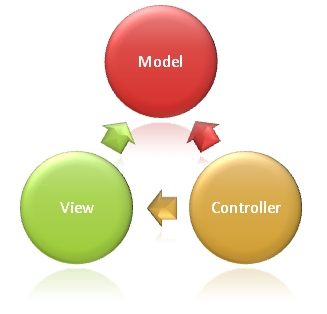
\includegraphics[width=0.5\linewidth]{assets/03_1.jpg}
	\caption{Schemat graficzny wzorca Model-Widok-Kontroler}
	\label{fig:mvc-pic}
\end{figure}

\subsection{Wzorzec Repozytorium} % (fold)
\label{sub:wzorzec_repozytorium}
\paragraph{} % (fold)
\label{par:}
\textit{Wzorzec Repozytorium} (\textit{Repository Pattern}) to popularna technika mająca na celu podział warstwy biznesowej na dwie części : \textit{Serwis} i \textit{Repozytorium}. \textit{Serwis} jest elementem odpowiedzialnym za logikę aplikacji oraz komunikację między kontrolerem, a repozytorium. \textit{Repozytorium} natomiast jest komponentem, ktorego zadanie polega na komunikacji z bazą danych : zapisywanie, pobieranie, edytowanie i usuwanie danych (model \textit{CRUD}). Takie rozsczepienie poszczególnych elementów pozwal na łatwe testowanie kodu, programowanie zorientowane na testy (\textit{ang. Test Driven Development}), szybką modernizację istniejącej logiki i rozbudowę aplikacji.

\paragraph{} % (fold)
\label{par:}
W projekcie \textit{Wzorzec Repozytorium} został zaimplementowany poprzez biblioteki \textbf{PI.Service (Serwis)} i \textbf{PI.Data (Repozytorium)}.
Dane z kontrolerów przekazywane są do \textit{Serwisu} pod postacią \textit{ViewModles} lub typów prymitywnych. \textbf{PI.Service} odpowiada za odpowiednią logikę przetwarzania danych, konwersji \textit{ViewModels} na \textit{Models} (przy wykorzystaniu narzędzia \textit{AutoMapper \footnote{AutoMapper - Sekcja \ref{sub:automapper}}}) i przekazaniu ich do \textit{Repozytorium}.

\paragraph{} % (fold)
\label{par:}
Funkcją biblioteki \textbf{PI.Data} jest odbieranie danych z \textit{Serwisu} i dokonanie odpowiednich operacji bazodanowych przy użyciu \textit{EntityFramework \footnote{EntityFramework - Sekcja \ref{sub:EntityFramework}}}

\paragraph{} % (fold)
\label{par:}
Schemat działania logiki biznesowej w oparciu o \textit{Wzorzec Repozytorium} został przedstawiony na Rysunku \ref{fig:repository-pattern} .

\begin{figure}[ht]
	\centering
		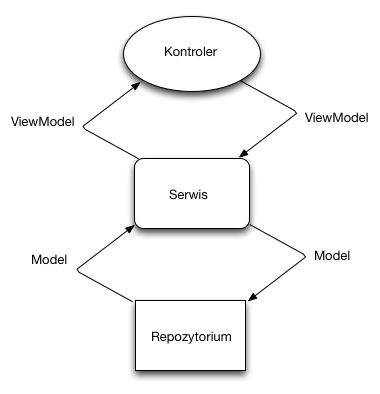
\includegraphics[width=0.8\linewidth]{assets/repository_pattern.png}
	\caption{Schemat przepływu danych przy wykorzystaniu Wzorca Repozytorium}
	\label{fig:repository-pattern}
\end{figure}

\subsection{Odwrócenie sterowania} % (fold)
\label{sub:odwr_cenie_sterowania}
\paragraph{} 
\textit{Odwrócenie sterowania} (\textit{ang. Inversion of Control}) to pradygmat odpowiedzialny za przeniesienie na zewnątrz obiektu odpowiedzialnego za kontrolę niektórych czynności. Termin ten jest często utożsamiany z \textit{Wstrzykiwaniem zależności (ang. Dependency Injection)}, jednak jest to tylko jedna z realizacji \textit{Odwrócenia sterowania}. 

\paragraph{} % (fold)
\label{par:}
\textit{Wstrzykiwanie zależności} zosatało zrealizowane w projekcie za pomocą biblioteki \textit{Unity \footnote{Unity - Sekcja \ref{sub:unity}}} na dwóch poziomach :
\begin{itemize}
	\item W warstwie Modelu - wszytstkie serwisy i repozytoria, oraz kontekst bazodanowy wstrzykiwane są jako parametry w konstruktorze
	\item W warstwie Kontrolorów - wstrzykiwany jest dostawca serwisów
\end{itemize} 

\paragraph{} % (fold)
\label{par:}
Takie rozdzielenie wstrzykiwania zależności pozwoliło na całkowite odseparowanie logiki bazodanowej i elementów za nią odpowiedzialnych od warstwy aplikacji.

\subsection{Bezpieczeństwo} % (fold)
\subsubsection{Autoryzacja}
\paragraph{} % (fold)
\label{par:paragraph_name}

% paragraph paragraph_name (end)
Do autoryzacji użytkowników, w projekcie wykorzystany zsotał popularny z technologii ASP.NET system \textit{Forms authentication}. \textit{Forms authentication} wykorzystuje znacznik uwierzytelniający, który zostaje utworzony w momencie gdy użytkownik zaloguje się na stronie. Zancznik \textit{Forms authentication} zwykle przechowywane jest wewnątrz szyfrowanego ciasteczka.

\paragraph{} % (fold)
\label{par:}
W momencie gdy użytkownik będzie chciał uzyskać dostęp do strony wymagającej uwierzytelnienia, a nie przechodził wcześniej procesu uwierzytelniania, zostanie przekierowany na zdefiniowaną w pliku konfiguracyjnym stronę logowania, na której będzie mógł wprowadzić nazwę użytkownika i hasło. Te dane są następnie przekazane do serwera, który sprawdza czy takowy użytkownik istnieje w bazie danych. Po pomyślnej weryfikacji danych, użytkownik zostaje uwierzytelniony, stworzony zostaje znacznik i następuje przekierowanie na stronę główną aplikacji.
% paragraph  (end)

\subsubsection{Przechowywanie hasła}
\paragraph{} % (fold)
\label{par:}
Przechowywane w systemie hasła, szyfrowane są poprzez wygenerowanie funkcji skrótu \textit{SHA-2} o wilekości 256 sklejonego z \textit{Solą} hasła. \textit{Sól} stanowi wygenerowany w momencie rejestracji \textit{GUID - identyfikator globalnie unikatowy}. W aplikacji został wykorzystany algorytm \textit{SHA-2}, ponieważ jest zancznie silniejszy od swoich poprzedników z rodziny \textit{SHA-1}, w którym zidentyfikowano luki w bezpieczeństwie. Ogólny algorytm szyfrowania wygląda następująco :

\paragraph{} % (fold)
\label{par:}

% paragraph  (end)
\lstset{language=Java,caption={Szyfrowanie hasła},label=DescriptiveLabel}

\begin{lstlisting}
		SHA256(concat(password,salt))
\end{lstlisting}

\paragraph{} % (fold)
\label{par:}
Dzięki zastosowaniu \textit{soli} zmniejszone zostaje prawdopodobieństwo złamania hasła popularnymi atakami : brutal force, atakiem słownikowym czy wykorzystującym tablice tęczowe.
% paragraph  (end)


\subsection{Wielojęzykowość} % (fold)
\label{sub:wieloj_zykowo_}
Dzięki zastosowaniu mechanizmu \textit{Zasobów (ang. Resource)} aplikacja internetowa jest dostosowana do szybkiego tłumaczenia na inne języki. Domyśnym językiem aplikacji jest angielski, a w obecnej wersji obsługuje również polski. By dodać inne tłumaczenie, należy stworzyć nowy plik \textit{resx}, o nazwie :

\lstset{language=Java,caption={Tłumaczenie aplikacji},label=DescriptiveLabel}
\begin{lstlisting}
			Main.xx.resx
\end{lstlisting}

\paragraph{} % (fold)
\label{par:}
gdzie \textit{xx} to dwuliterowy skrót języka przeglądarki, w którym należy umieścić odopwiednie wartość dla podaych kluczy.
% paragraph  (end)

\subsection{Azure} % (fold)
\label{sub:azure}
\paragraph{} % (fold)
\label{par:}
Aplikacja została przystosowana do natychmiastowej możliwośći wdrożenia na platformę Windows Azure SDK. W tym celu należy dokonać publikacji projektu o nazwie \textbf{PI.Azure} oraz zaimportować go jak serwis lub stronę w portalu http://windos.azure.com .
% paragraph  (end)
% subsection azure (end)

\section{Baza Danych} % (fold)
\label{sec:baza_danych}
\paragraph{} % (fold)
\label{par:}
Baza danych, do której dostęp ma aplikacja internetowa działa na serwerze \textit{Microsoft SQL Server 2012 \footnote{MS SQL 2012 - Sekcja \ref{sub:mssql}}}. Do zarządzania danymi wykorzystany został wykorzystana bibliotek \textit{EntityFramework \footnote{EntityFramework - Sekcja \ref{sub:EntityFramework}}}. W bazie danych przechowywane są informacje o profilu użytkownika,treningach, wiadomościach, logach, ustawieniach konta oraz zarejestrowane przez aplikację mobilną współrzędne GPS.

\paragraph{} % (fold)
\label{par:}
W tworzeniu i zarządzaniu bazą danych wykorzystane zostało podejście \textit{Code First}, polegające na modelowaniu bazy danych pod postacią klas języka \textit{C\#}, a następnie wygenerowaniu gotowej bazy danych przy pomocy EntityFramework. By zabezpieczyć dane składowane w bazie danych przed usunięciem ich w wyniku zmiany modelu w kodzie projektu, użyty został mechanizm migracji. 
Schemat bazy danych przedstawiony został na Rysunku \ref{fig:database} .


\label{sub:schemat_bazy_danych}
\begin{figure}[ht]
	\centering
		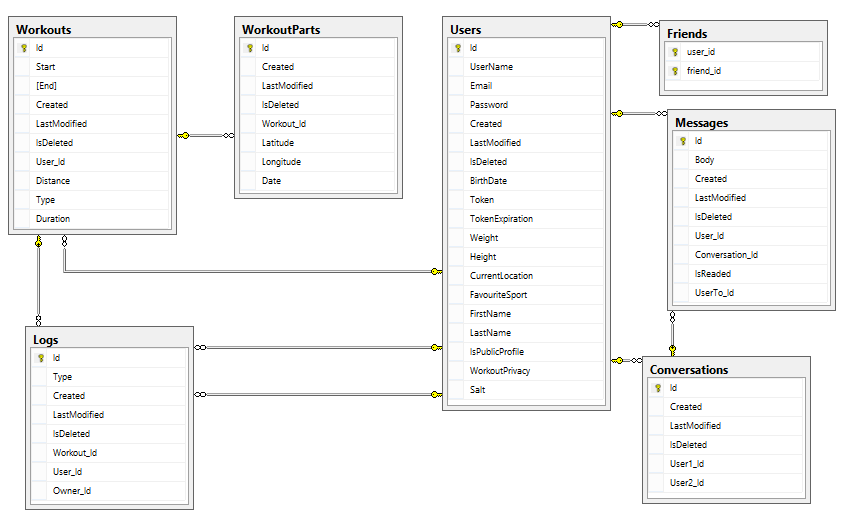
\includegraphics[width=1\linewidth]{assets/database.png}
	\caption{Schemat bazy danych}
	\label{fig:database}
\end{figure}

% subsection schemat_bazy_danych (end)
% paragraph  (end)

% section baza_danych (end)
\newpage
\section{Warstwa prezentacji} % (fold)
\label{sec:warstwa_aplikacji}
\paragraph{} % (fold)
\label{par:}
By aplikacja internetowa była przyjazna i łatwa w użyciu, należy zadbać o przejrzysty, łatwy w obsłudze i estetyczny interfejs. W tym celu wykorzystana została popularna biblioteka stylów CSS Twitter-Bootstrap \footnote{http://twitter.github.com/bootstrap/}. Dzięki dużej ilośći gotowych komponentów, można w łatwy i szybki sposób projektować wygląd strony internetowej, spełniający oczekiwania współczesnego użytkownika. Twitter-Bootstrap to nie tylko biblioteka styli CSS, ale również zbiór elementów JavaScript takich jak okna modalne czy zakładki.

\paragraph{} % (fold)
\label{par:}
W celu poprawienia funkcjonalności aplikacji i interakcji z użytkownikiem wykorzystane zotały dodatkowe moduły takie jak :
\begin{itemize}
\item jQuery Data Table \footnote{http://datatables.net/}
\item pNotify \footnote{http://pinesframework.org/pnotify/}
\item jQuery DatePicker \footnote{http://jqueryui.com/}
\item jQuery DateTimePicker \footnote{http://trentrichardson.com/examples/timepicker/}
\item FullCalendar \footnote{http://arshaw.com/fullcalendar/}
\item Google Maps JavaScript API v3 \footnote{https://developers.google.com/maps/documentation/javascript/}
\end{itemize}


\section{Funkcjonalności} % (fold)
\label{sec:funkcjonalno_ci}

\subsection{Treningi} % (fold)
\label{sub:treningi}

\paragraph{}
Moduł do obsługi treningów jest najważniejszym elementem projektu. Pozwala on na śledzenie dodawanie i archiwizowanie danych dotyczących. Zapisane w systemie treningi wyświetlane są na kalendarzu (Rysunek \ref{fig:workout_main}), przez co można w uporządkowany sposób zarządzać treningami, planować następne sesje, archiwizować dane i wyszukiwać wcześniejsze rekordy. Po kliknięciu na wybrany przez nas trening, wyświetlone zostaje modalne okno zawierjące wszystkie inforamcje dotyczące aktywności : typ, data początku i końca, czas, dystans i jeżeli w bazie danych są przechowane współrzędne GPS, to również mapa z zaznaczoną trasą (Rysunek \ref{fig:workout_map}).
\paragraph{} % (fold)
\label{par:}

% paragraph  (end)
 Dodawanie treningu może odbywać się na dwa sposoby : poprzez synchronizację z danymi przechowywanymi przez aplikację mobilną lub dodając rekord bezpośrednio poprzez interfejs aplikacji internetowej (Rysunek \ref{fig:add_workout}).


\begin{figure}[ht]
	\centering
		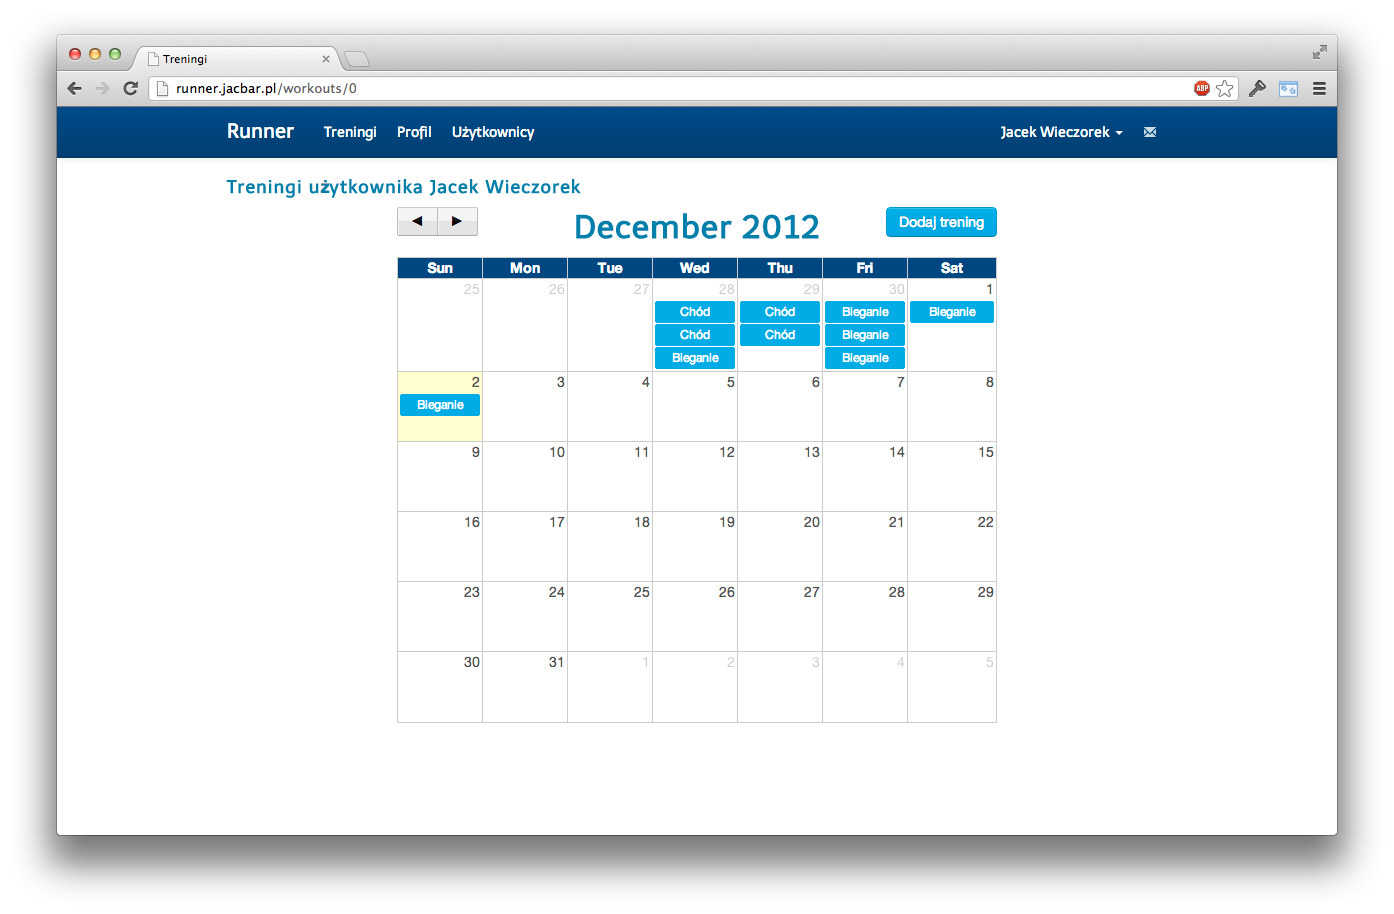
\includegraphics[width=1\linewidth]{assets/workouts_main.png}
	\caption{Widok strony agregującej dodane rekordy}
	\label{fig:workout_main}
\end{figure}

\begin{figure}[ht]
	\centering
		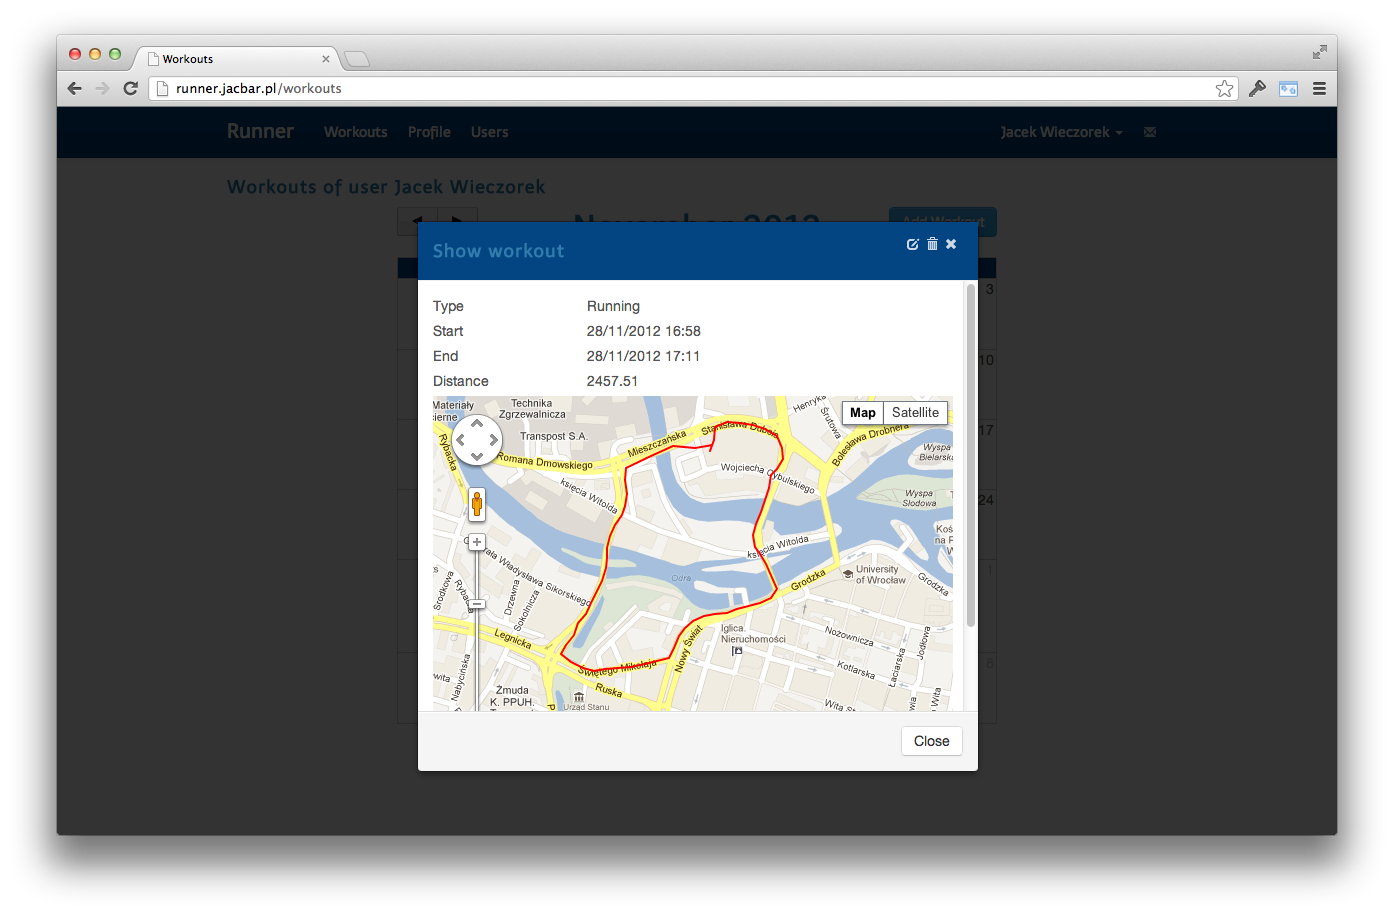
\includegraphics[width=1\linewidth]{assets/workout_map.png}
	\caption{Widok treningu z zaznaczoną trasą}
	\label{fig:workout_map}
\end{figure}

\begin{figure}[ht]
	\centering
		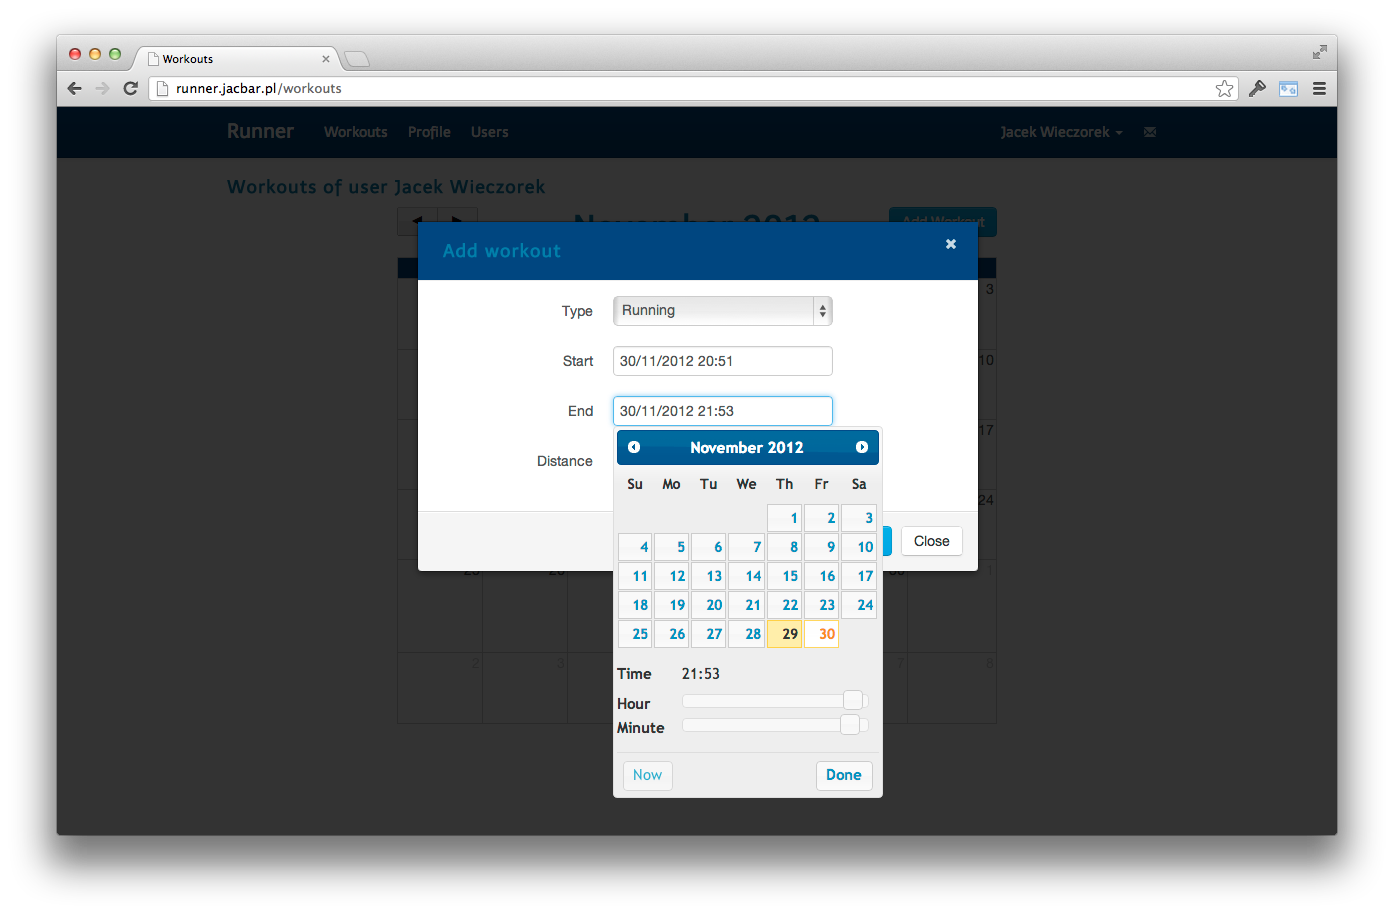
\includegraphics[width=1\linewidth]{assets/add_workout2.png}
	\caption{Dodawanie treningu poprzez aplikację internetową}
	\label{fig:add_workout}
\end{figure}

\section{Funkcje portalu społecznościowego} % (fold)
\label{sec:profil_u_ytkownika}
\paragraph{} % (fold)
\label{par:}
By zapewnić powodzenie aplikacji w dzisiejszych czasach należy zadbać również o dodatkowe funkcjonalności aplikacji, pozwalające na interakcję z użytkowników między sobą. Możliwość podąrzania za użytkownikami, przeglądanie ich aktywności, osiągnięć, możliwość komunikacji poprzez wysyłanie wiadomości sprawia, iż aplikacja staje się małym portalem społecznościowym. 
\paragraph{} % (fold)
\label{par:}

% paragraph  (end)
Jednak by zadowolić użytkowników, chcących wykorzystywać serwis tylko i wyłącznie jako internetowy dziennik treningów, zaimplementowane zostały różne poziomy udostępniania treści innym osobom korzystającym z portalu. Podstawowe wiadomości jak imię i nazwisko oraz nazwa użytkownika są widoczne dla wszystkich, jednak resztę informacji w tym adres email można ukryć, wyłączając w widoku edycji profilu flagę "Profil publiczny". Również istnieje możliwość udostępniania swoich treningów innym użytkownikom na trzech poziomach : dostępne dla wszytskich, dostępne dla użytkowników podążających, niewidoczne dla nikogo.
% paragraph  (end)


